\chapter{Экспериментальный раздел}
\label{cha:research}
    В данном разделе будут проведены эксперименты для проведения 
    сравнительного анализа алгоритмов по затрачиваемому процессорному 
    времени в зависимости от длины массива и степени его отсортированности.

    \section{Сравнительный анализ на основе замеров времени работы алгоритмов}
        В рамках данного проекта были проведёны следующие эксперименты:

        1) сравнение времени работы параллельного нечёткого алгоритма k-means при разном количестве потоков(график \ref{graph:test:1});
        
        2) сравнение времени работы параллельного и последовательного нечёткого алгоритма k-means при разном размере массива(график \ref{graph:test:2}).

        
        Тестирование проводилось на компьютере с процессором
        Intel(R) Core(TM) i5-8265U CPU @ 1.60GHz 1.80 GHz под управлением Windows 11 с 8 Гб оперативной памяти.\\

        \begin{figure}[h!]
            \centering
            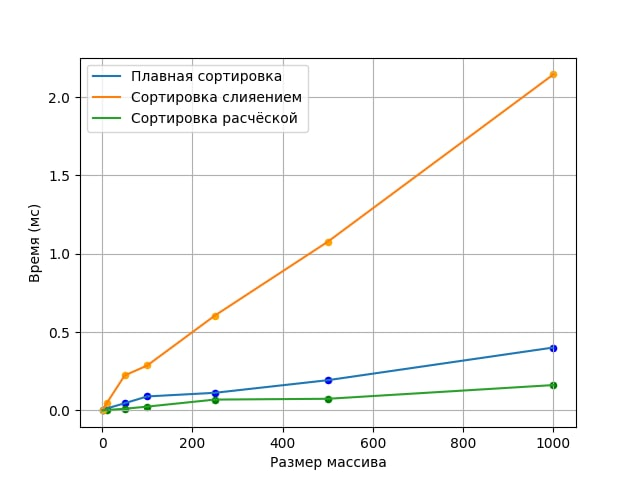
\includegraphics[scale=0.9]{graph_1.png}
            \caption{Зависимость времени работы параллельного нечеткого алгоритма k-means от количества потоков}
            \label{graph:test:1}
        \end{figure}
        \newpage
        \begin{figure}[h!]
            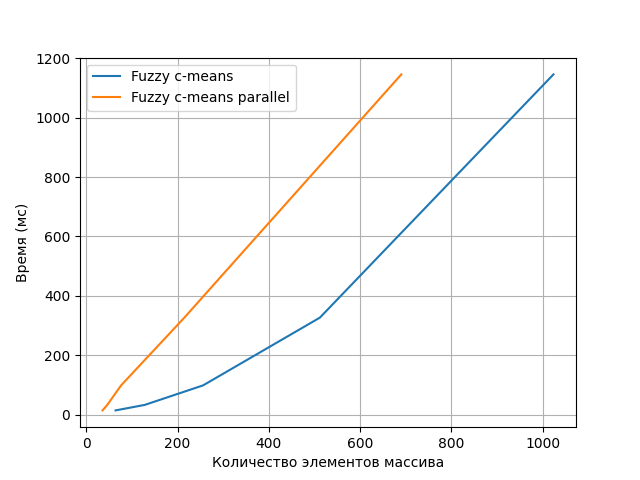
\includegraphics[scale=0.9]{graph_2.png}
            \caption{Зависимость времени работы параллельного и последовательного нечеткого алгоритма k-means от размера массива (количество потоков -- 4)}
            \label{graph:test:2}
        \end{figure}
        \newpage


    \section{Вывод}
        \par В ходе экспериментов по замеру времени работы было установлено, что в параллельный нечёткий алгоритм дает наиболее быстрый результат при количестве потоков равному количеству логических ядер компьютера.
        \par Также было установлено, что параллельный алгоритм при любом размере массива работает быстрее последовательного алгоритма.


\newpage